
%(BEGIN_QUESTION)
% Copyright 2008, Tony R. Kuphaldt, released under the Creative Commons Attribution License (v 1.0)
% This means you may do almost anything with this work of mine, so long as you give me proper credit

A {\it centrifugal pump} works by spinning a disk with radial vanes called an ``impeller,'' which flings fluid outward from the center of the disk to the edge of the disk.  This kinetic energy imparted to the fluid translates to potential energy in the form of pressure when the fluid molecules strike the inner wall of the pump casing:

$$\includegraphics[width=15.5cm]{i01407x03.eps}$$

The performance of a centrifugal pump is often expressed in a special graph known as a {\it pump curve}.  A typical centrifugal pump curve appears here:

$$\includegraphics[width=15.5cm]{i01407x01.eps}$$

Examine this pump curve, and explain in your own words what it tells us about the performance behavior of this pump.

\vskip 20pt \vbox{\hrule \hbox{\strut \vrule{} {\bf Suggestions for Socratic discussion} \vrule} \hrule}

\begin{itemize}
\item{} One way to describe the operation of a centrifugal pump is to say it generates discharge pressure by converting kinetic energy into potential energy.  Elaborate on this statement, explaining exactly where and how kinetic energy gets converted to potential energy.  Hint: this might be easier to answer if you consider the ``limiting case'' of maximum discharge pressure described by the pump curve, where flow is zero and pressure is maximum.
\item{} Appealing to the conversion of energy between kinetic and potential forms, explain {\it why} discharge pressure for a centrifugal pump falls off as flow rate increases.
\item{} The pump curve shown assumes a constant rotational speed for the pump's impeller.  How would the pump curve be modified if the pump were rotated at a slower speed?
\end{itemize}

\underbar{file i01407}
%(END_QUESTION)





%(BEGIN_ANSWER)

This graph relates pressure output versus liquid flow rate for a centrifugal-style pump operating at a constant rotational speed.
 
%(END_ANSWER)





%(BEGIN_NOTES)

A {\it pump curve} is a graph of pressure output versus liquid flow rate for a centrifugal-style pump operating at a constant rotational speed.  Pump curves are essential for calculating precise pressure and flow values in liquid pumping systems.

\vskip 10pt

Centrifugal pumps are {\it inertial} in nature.  They work by imparting kinetic energy to the fluid molecules, not by moving fixed volumes of fluid for each rotation as is the case (by definition) for a positive displacement pump.  One way to envision the difference is to ask yourself whether or not fluid can flow freely through the pump mechanism by means of some external pressure source, if the pump shaft were to seize and become immobile.  For a true positive displacement pump, fluid flow would become blocked: no shaft motion means fluid volume {\it cannot} pass through the pump.

\vskip 10pt

A positive displacement pump spun at constant speed will pump a constant flow rate regardless of pressure.  Therefore, the ideal pump curve for a positive-displacement pump is a vertical line:

$$\includegraphics[width=15.5cm]{i01407x02.eps}$$

The real pump curve for a positive displacement pump will bend slightly at the top (toward the left) owning to internal leakage with increasing pressure.

\vfil \eject

\noindent
{\bf Prep Quiz:}

A {\it pump curve} describes:

\begin{itemize}
\item{} The proper bend radii for pipe elbows before and after a pump
\vskip 5pt 
\item{} The curvature of the flow path as fluid enters the pump casing
\vskip 5pt 
\item{} The pressure versus flow characteristics of a pump
\vskip 5pt 
\item{} The amount of fluid turbulence inside a pump at different speeds
\vskip 5pt 
\item{} The maximum density of fluid that a pump is able to handle
\vskip 5pt 
\item{} The power requirements of the pump at different fluid densities
\end{itemize}


%INDEX% Final Control Elements, pump: pressure/flow curve
%INDEX% Machine, centrifugal pump

%(END_NOTES)


